This sections evaluates the performance of proposed methodology in estimating correspondences of human poses in-the-wild. Results for quantitative an qualitative experiments are reported. Experiments \ref{exp:internal} investigate the accuracy of estimating dense correspondences of non-rigid deformable objects, and the impact of annotating outlines of human poses instead of annotating skeletons. Experiments \ref{exp:benchmark} compare the joints localisation accuracy of our skeleton prediction from outline fitting with respect to that of state-of-the-art human pose estimation algorithms in-the-wild. Note that all results reported in this section were obtained by fitting Patch AAM using the fast version of the Simultaneous Inverse Compositional algorithm (Fast-SIC) originally proposed by the authors of \cite{Papandreou2008}. For further experimental results and visualisations please refer to our supplementary material.

\subsection{Databases \& Error Metrics}
There are significant numbers of datasets exist for human pose estimation, where FLIC\cite{sapp2013modec}, BBC Pose\cite{pfister2015flowing}, Fashion Pose\cite{dantone2013human} and MPII\cite{andriluka14cvpr} attracted most public attention. In our work, we reported our performance comparison on BBC Pose Dataset\cite{pfister2015flowing}, which has relatively most consistent skeleton annotation among the others.

The training of dense Active Appearance Models (dAAMs) for upper body involves manual outline annotation from a combination of datasets, including H3D\cite{PoseletsICCV09}, Microsoft COCO\cite{lin2014microsoft}, MPII\cite{andriluka14cvpr}, Fashion Pose\cite{dantone2013human}, FLIC\cite{sapp2013modec} and BBC Poses\cite{pfister2015flowing}. The training set contains 891 training images from where 500 are annotated with outline manually. A dAAMs is built from 500 training images thereby produces dense correspondences for generating sparse outline annotation (29 landmarks). A Patch AAM is build from sparse annotations before fitting to 391 images. Manual minor correction are required for putting those fitted image to training set. The final Patch AAM is built from 891 images and validated on validation set given by BBC Pose.

In order to compare with current state-of-the-art human pose estimation on BBC Pose, we uses same error metric as BBC Poses does, which normalises testing images to have height of 256 pixels. Performance measure of experiments in this paper are plot with Cumulative Error Distribution (CED) curve, where graph shows accuracy against distance from ground truth in pixels on normalised images.

\subsection{Benchmark Against State-of-the-art}
\label{exp:benchmark}
This experiment presented the accuracy of predicting joints positions from establishing dense correspondences with outline fitting. We build Patch AAM using 891 training hand images from a combination of datasets, where each image has 29 landmarks annotated alone its boundary. Dense scale-invariant feature transform (DSIFT)\cite{PoseletsICCV09} feature is used from image representation for our model. Model fitting is initialised based on current state-of-the-art human pose estimation algorithms on BBC Pose dataset. Results for this experiment are reported over 1000 testing images BBC Pose Provided, which human upper-body pose are landmark with 7 points on skeleton. For our model, joints are projected from the dense correspondence generated from our proposed method.

Cumulative Error Distributions (CED) for this experiment are shown in Figure \ref{fig:hand_benchmark} while fitting statistics are reported in Table \ref{tab:hand_benchmark}. Results show that, for this experiment, the fitting accuracy achieved by our method outperformed current state-of-the-art algorithms. In particular, our method improves performance of current best method \cite{pfister2015flowing} by a notable amount (9\% with error less than 6pt) on wrist, as well as marginal improvement on elbow estimation.


\begin{figure}[b!]
    \centering
    \begin{subfigure}[b]{0.23\textwidth}
            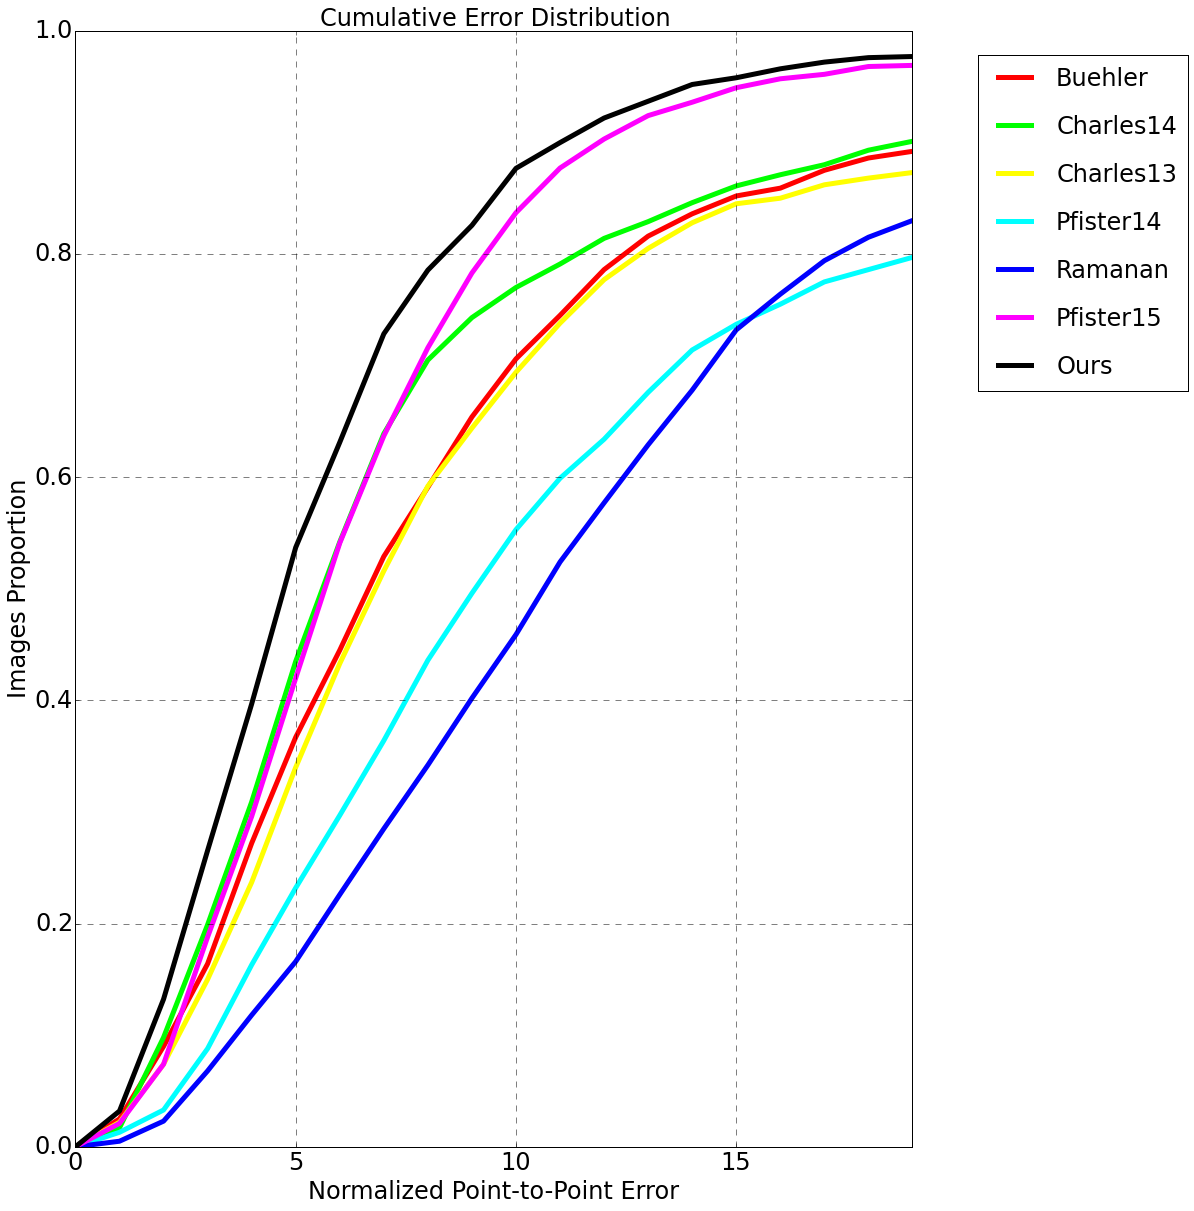
\includegraphics[width=\textwidth]{resources/HandBenchmark/wrist}
    \end{subfigure}
    \hfill
    \begin{subfigure}[b]{0.23\textwidth}
            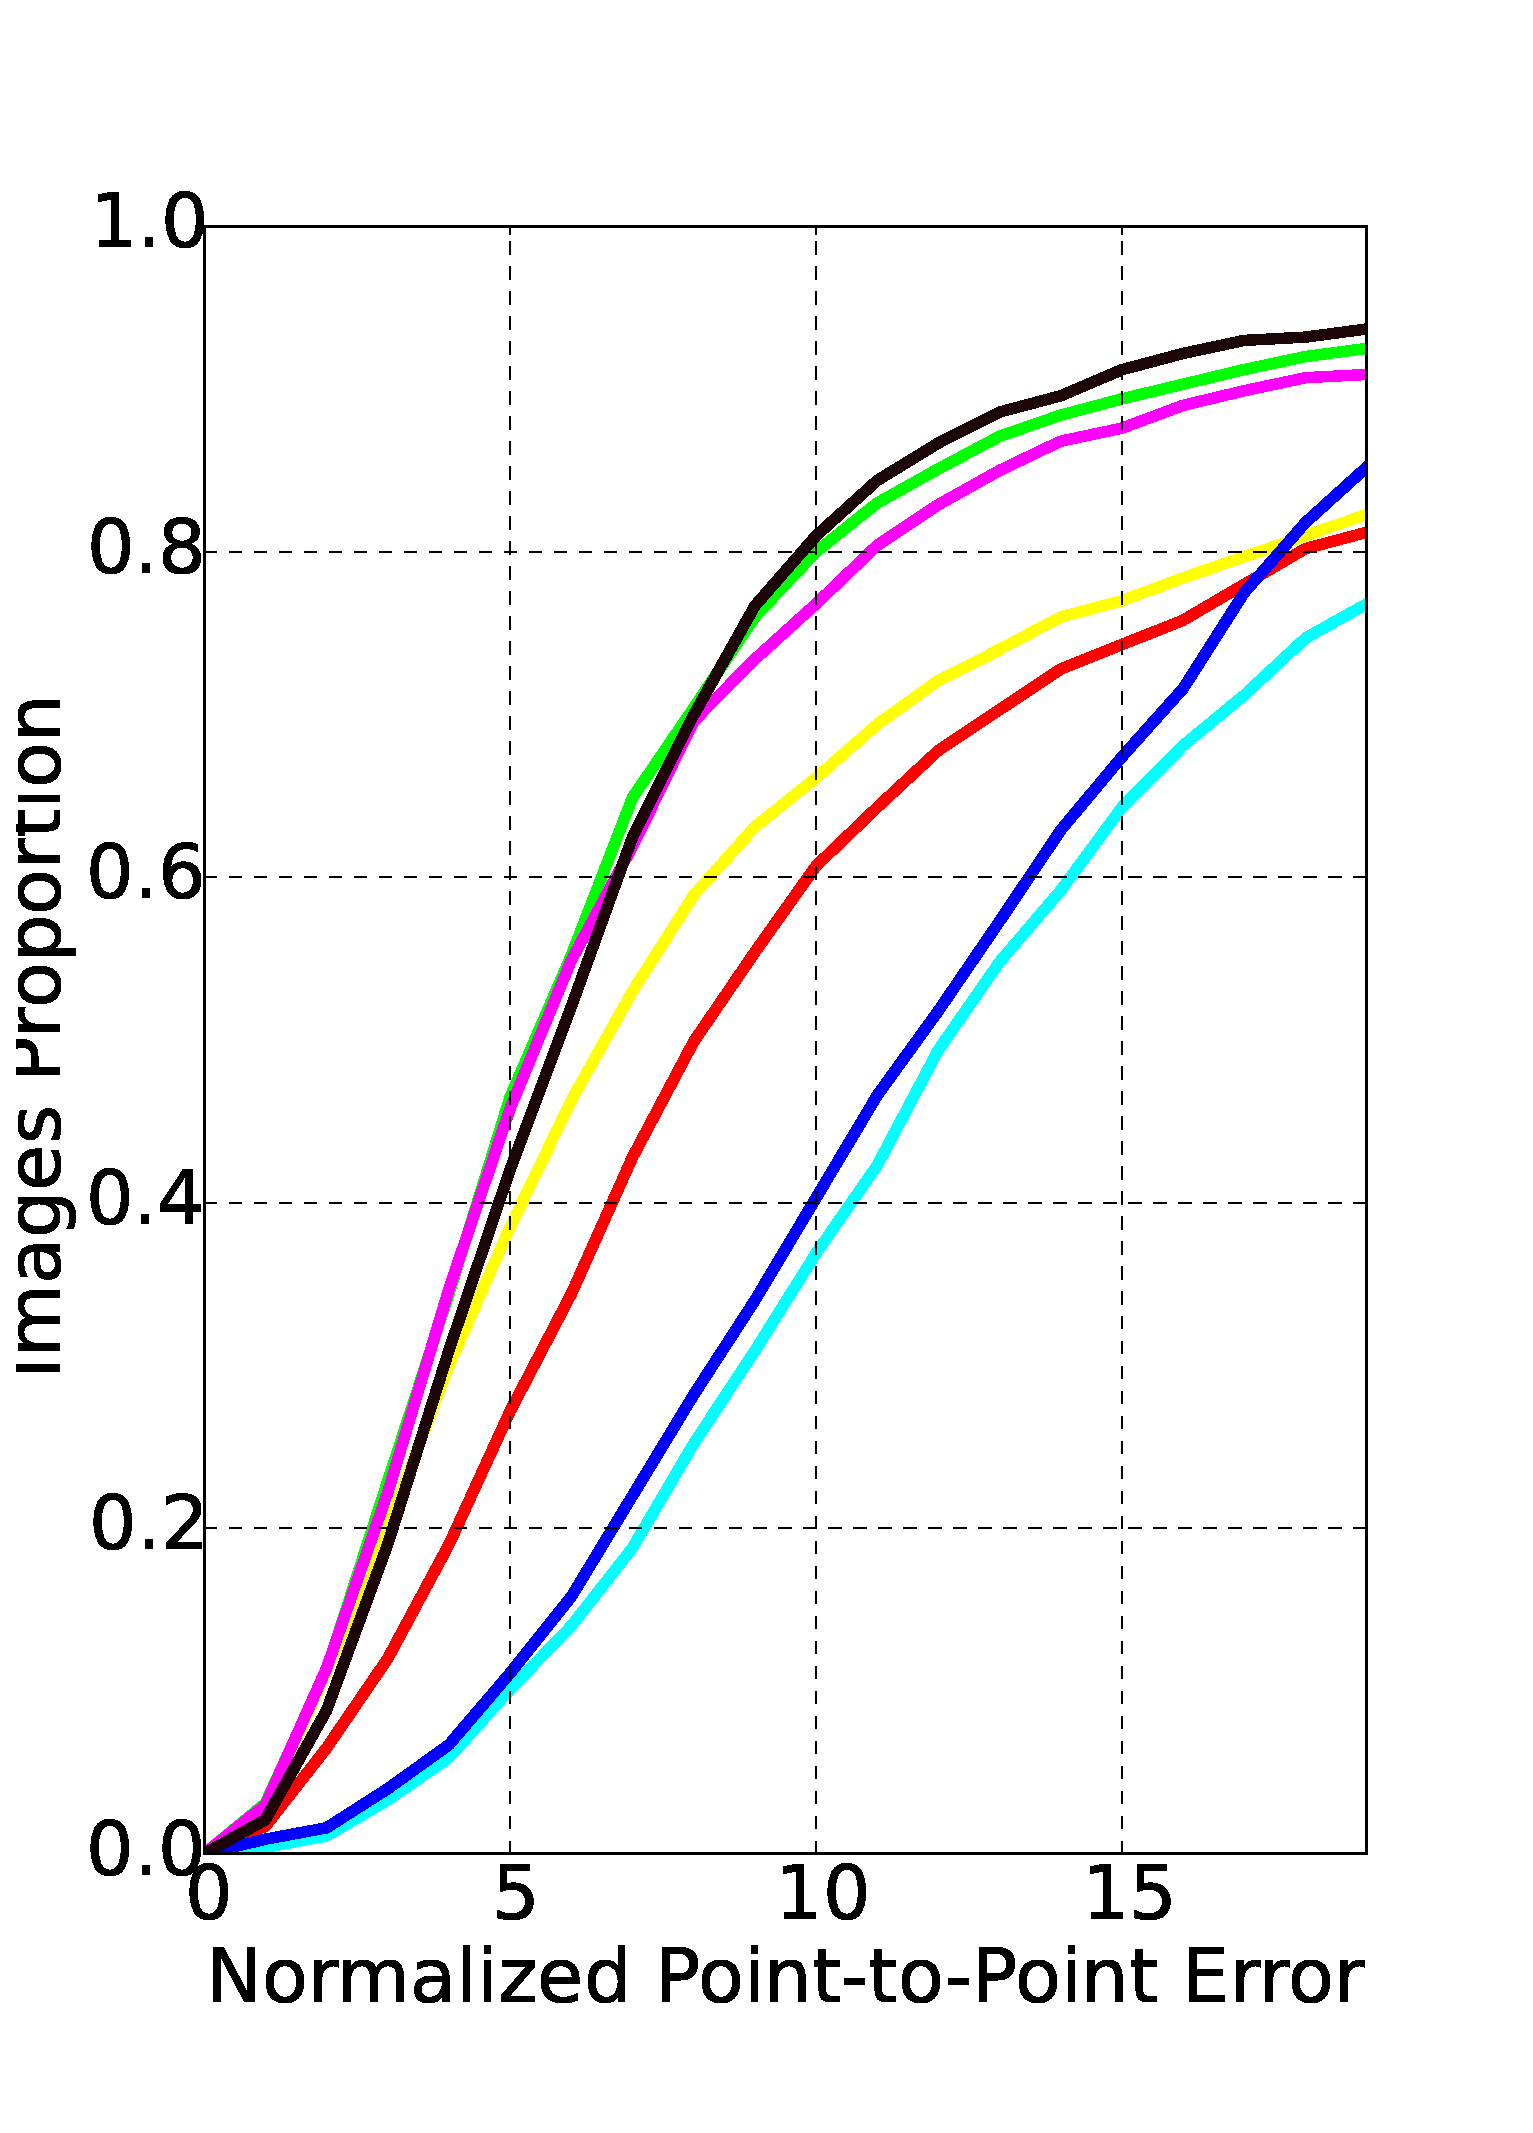
\includegraphics[width=\textwidth]{resources/HandBenchmark/elbow}
    \end{subfigure}
    \caption{CEDs over skeleton landmarks on BBC Pose database for experiment \ref{exp:benchmark}}
    \label{fig:hand_benchmark}
\end{figure}


\begin{table}[b!]
    \small
    \centering
    \begin{tabular}{|l|c|c|c||c|c|c|}
        \hline
                            & \multicolumn{3}{c||}{Wrist} & \multicolumn{3}{c|}{Elbow}\\
        \hline
        \emph{Method}       & \emph{mean} & \emph{std} & $\leq 6pt$ & \emph{mean} & \emph{std} & $\leq 6pt$\\
        \hline\hline
        Buehler             & 12.08    & 19.94        & 44.5\%       & 12.94    & 14.65        & 34.4\%\\
        Charles14           & 11.81    & 20.89        & 54.2\%       &  8.30    & 11.00        & \textbf{55.2\%}\\
        Charles13           & 13.78    & 22.39        & 43.3\%       & 13.17    & 18.74        & 46.3\%\\
        Pfister14           & 14.69    & 17.89        & 29.7\%       & 14.60    & 10.59        & 14.0\%\\
        Ramanan             & 15.59    & 19.04        & 22.6\%       & 15.53    & 10.82        & 15.8\%\\
        Pfister15           & 7.62     & 11.04        & 54.1\%       &  8.84    & 11.44        & 54.9\%\\
        \hline\hline
        Ours                & \textbf{6.791}& \textbf{10.910}   & \textbf{63.1\%}       & \textbf{8.250}     &  \textbf{10.564}        & 52.1\%\\
        \hline
    \end{tabular}
    \caption{Fitting statistics on BBC Pose database for experiment \ref{exp:benchmark}}
    \label{tab:hand_benchmark}
\end{table}


\subsection{Internal Evaluation}
\label{exp:internal}

\begin{figure}[t!]
    \centering
    \begin{subfigure}[b]{0.23\textwidth}
            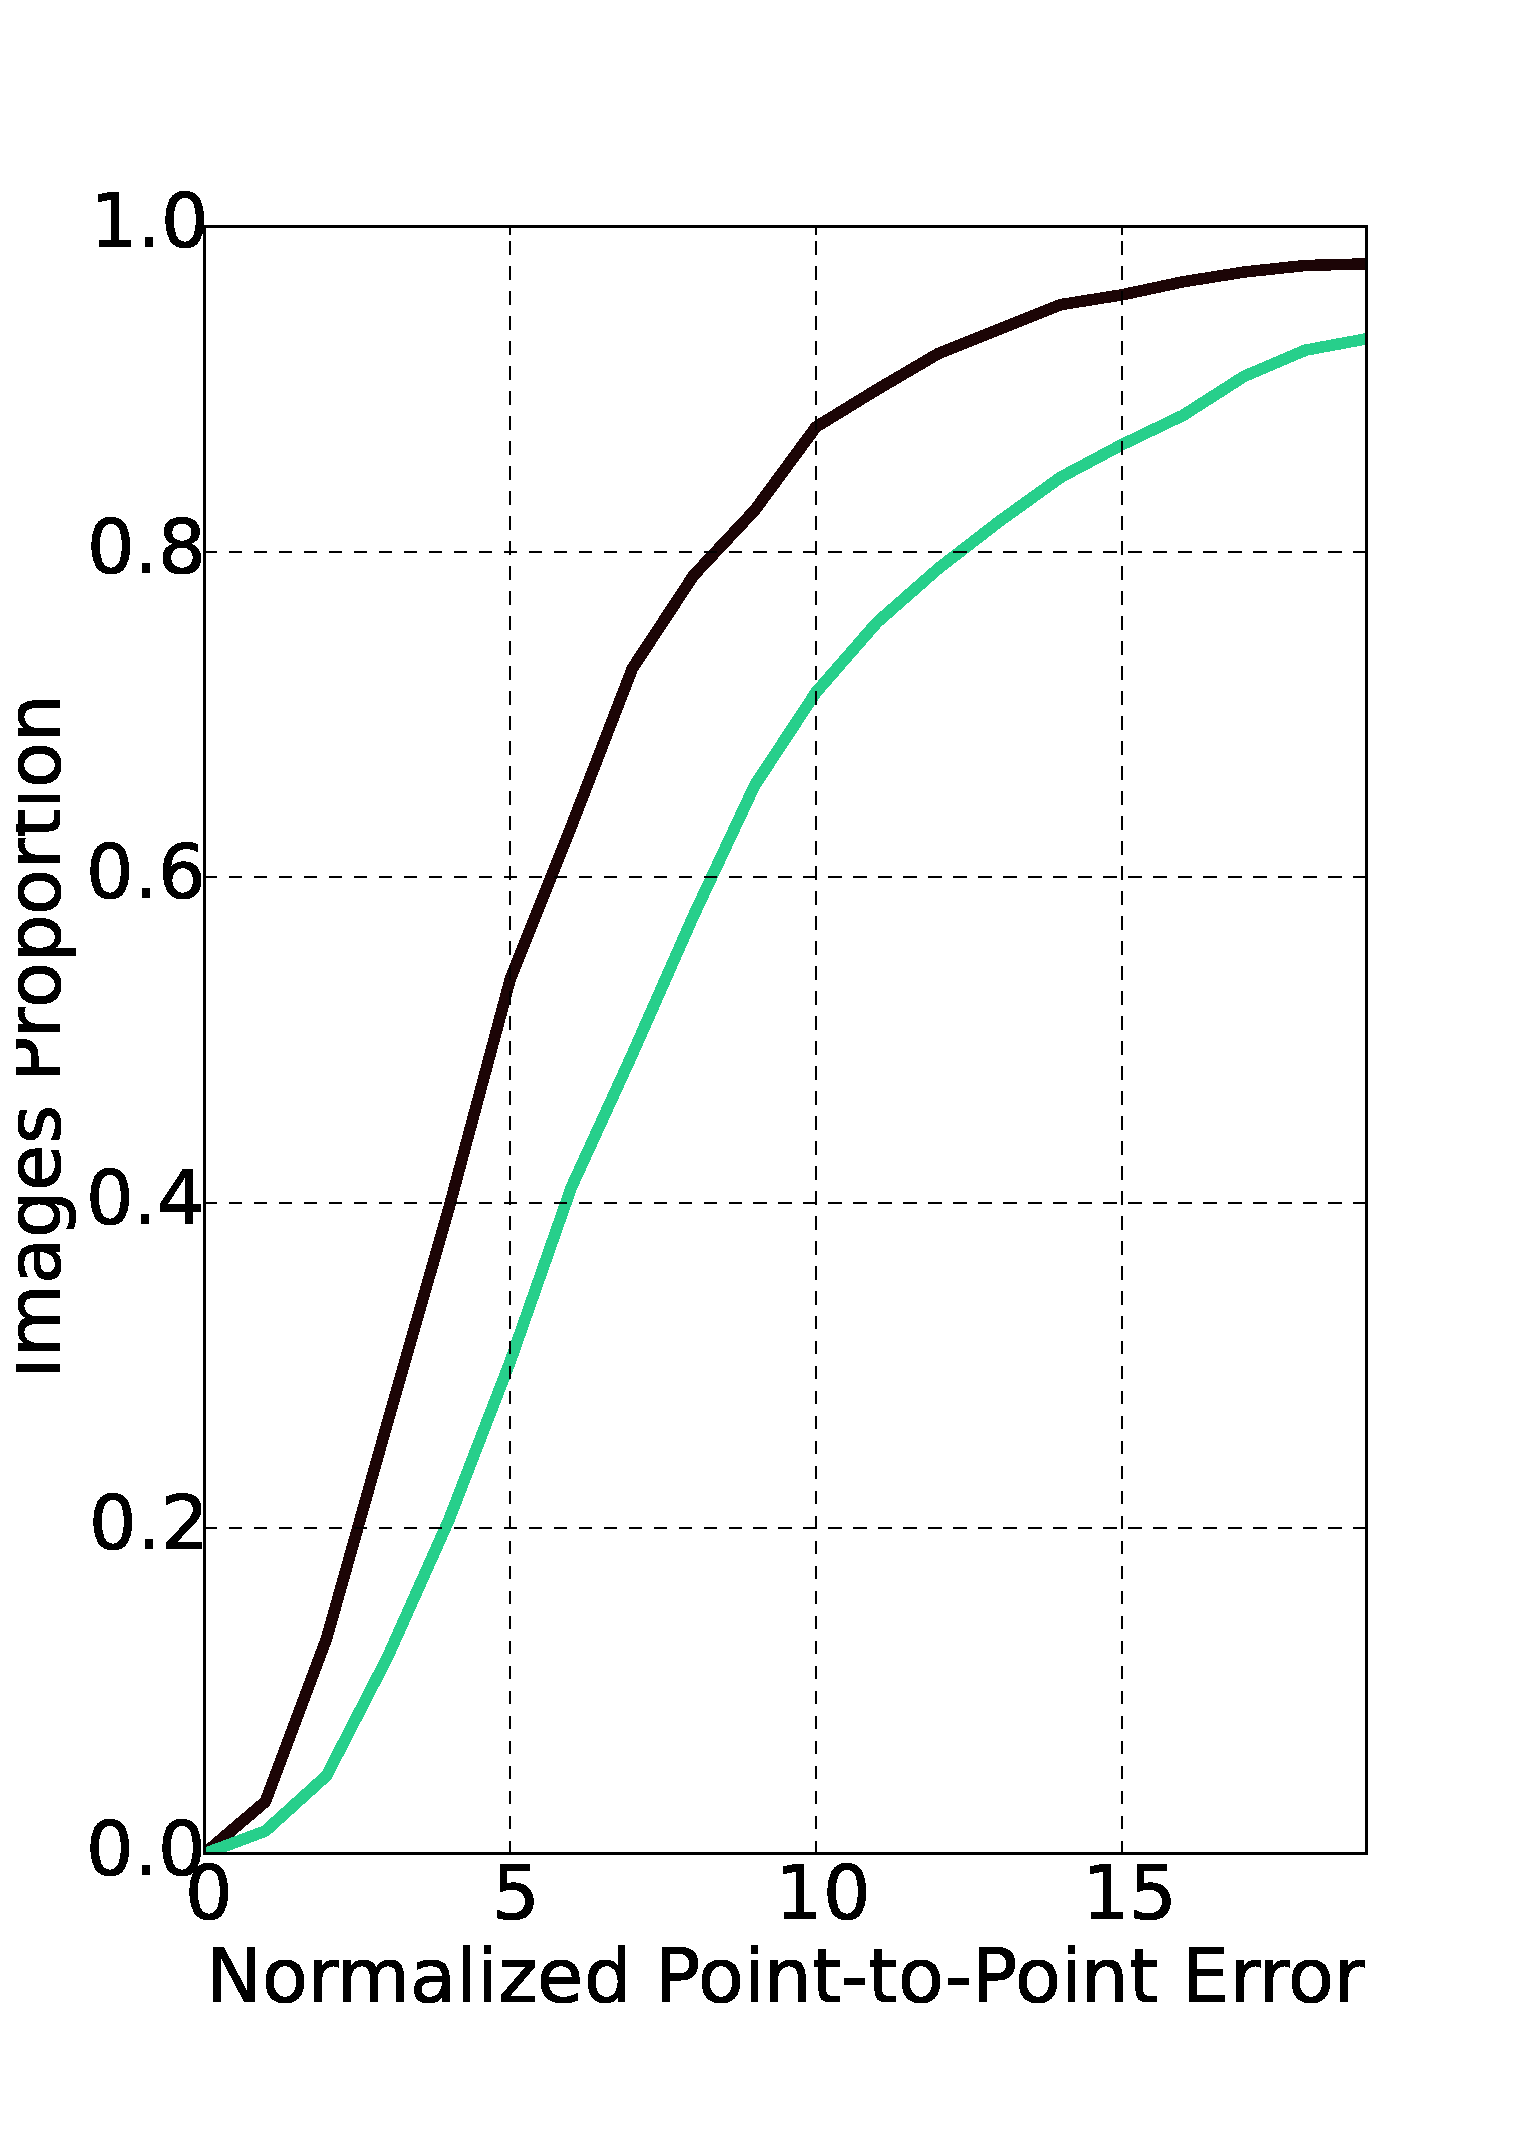
\includegraphics[width=\textwidth]{resources/HandBenchmark/elbow_joints}
    \end{subfigure}
    \hfill
    \begin{subfigure}[b]{0.23\textwidth}
            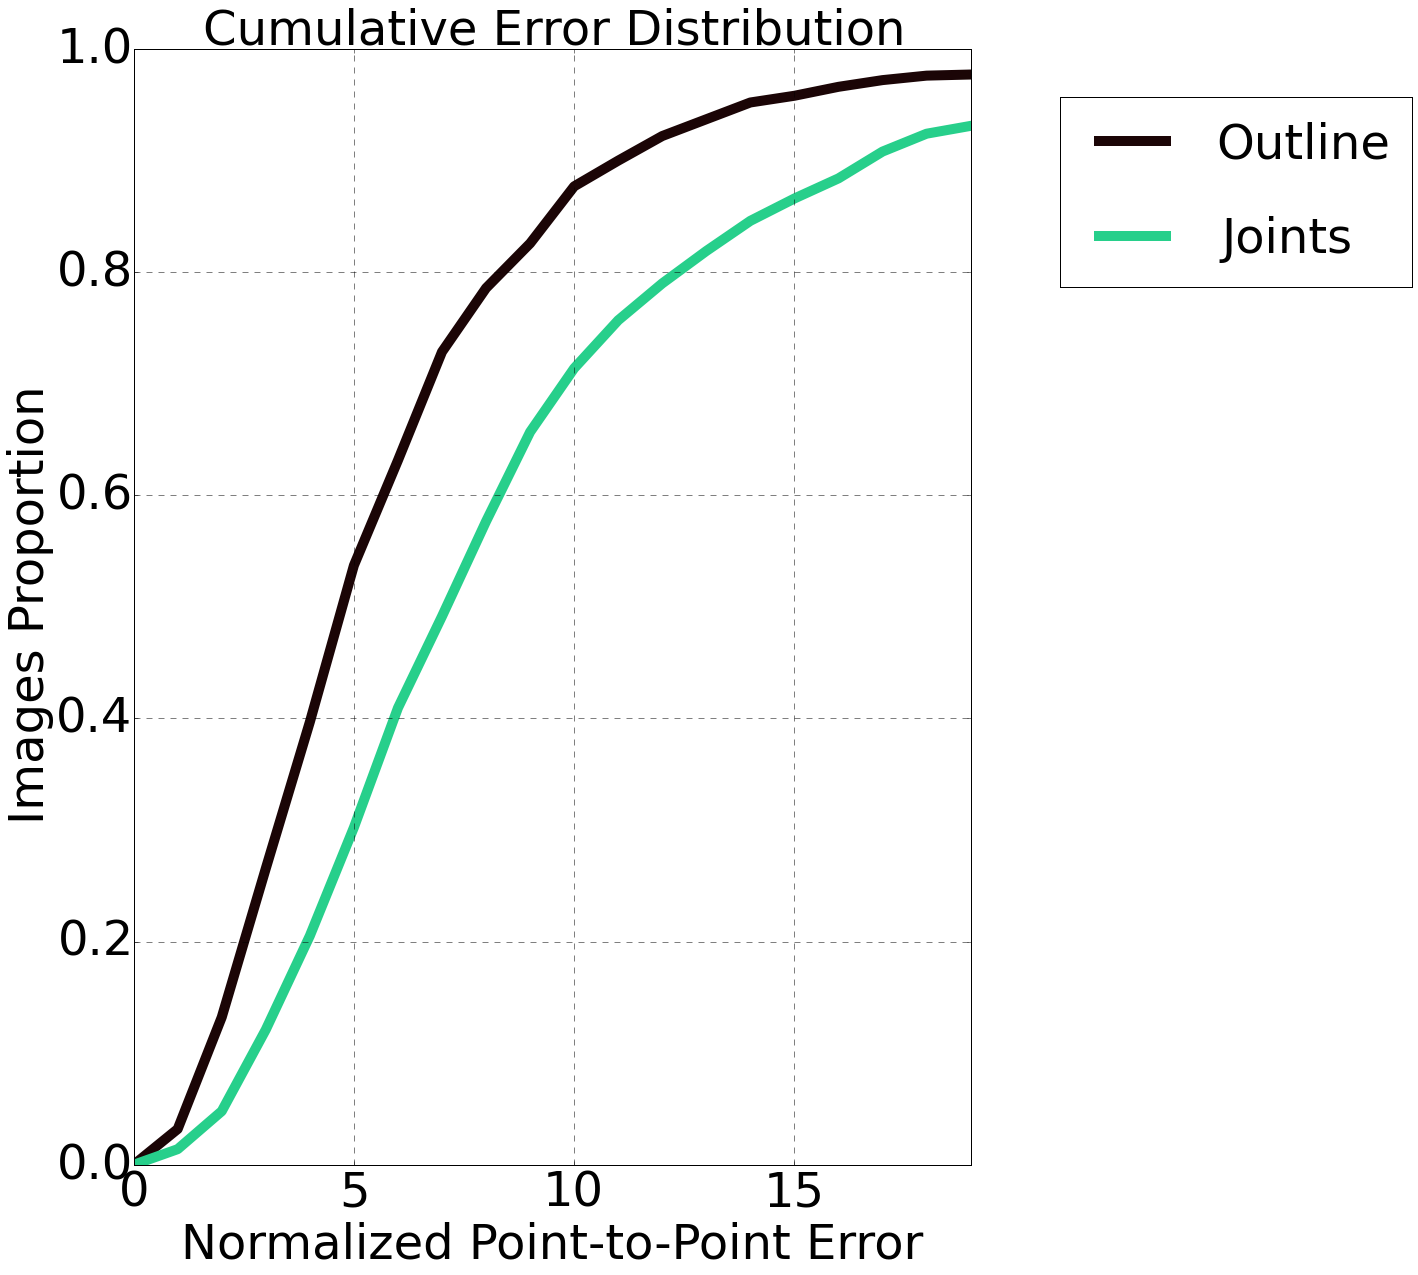
\includegraphics[width=\textwidth]{resources/HandBenchmark/wrist_joints}
    \end{subfigure}
    \caption{Hand Benchmark.}
    \label{fig:internal_benchmark}
\end{figure}


\subsection{Qualitative Results}
\label{exp:qualitative}
